\documentclass{article}
\usepackage[utf8]{inputenc}
\usepackage{amsmath}
\usepackage{amsfonts}
\usepackage{setspace}
\usepackage{amsthm}
\usepackage{amssymb}
\usepackage{geometry}
\usepackage{mathrsfs}
\geometry{left=3cm,right=3cm,top=2.25cm,bottom=2.25cm} 
\usepackage{graphicx}
\usepackage[ruled,lined,commentsnumbered]{algorithm2e}
\usepackage{bbm}
\usepackage{subfigure}
\usepackage{tikz}

\renewcommand{\qedsymbol}{\hfill $\blacksquare$\par}
\newcommand{\whiteqed}{\hfill $\square$\par}
\newcommand{\set}[1]{\left\{#1\right\}}
\newenvironment{solution}{\begin{proof}[\noindent\it Solution]}{\end{proof}}
\newenvironment{disproof}{\begin{proof}[\noindent\it Disproof]}{\end{proof}}
\newcommand{\staExp}[2]{\mathbb{E}_{#1}\left[#2\right]}
\renewcommand{\Pr}[2]{\mathbf{Pr}_{#1}\left[#2\right]}
\newcommand{\bd}[1]{\boldsymbol{#1}}

\allowdisplaybreaks[4]
\setstretch{1.5}


\title{\textbf{Data Mining Homework 01}}
\author{Qiu Yihang}
\date{March 2023}

\begin{document}


\maketitle

\vspace{1em}
\section{Whether Distances are Metrics}
\vspace{1em}
\subsection{Jaccard Distance is A Metric}
\vspace{1em}
\begin{proof}

    Recall that Jaccard Distance is 

    \vspace{-0.75em}
    $$d(C_1,C_2)=1-\dfrac{|C_1\cap C_2|}{|C_1\cup C_2|}$$

    \hspace{1.3em}
    \textbf{Property 1.} For any set $A,B$, $|A\cap B|\le|A\cup B|$, i.e. $\dfrac{|A\cap B|}{|A\cup B|}\le 1$. Thus, $d(A,B)\geq0.$

    \vspace{1em} \hspace{1.3em}
    \textbf{Property 2.} $d(A,B)=0$ \textbf{iff.} $A=B$. The proof is as follows.

    \vspace{-3em}
    \begin{align*}
        A=B &\Longrightarrow |A\cup B|=|A\cap B| \Longrightarrow d(A,B)=0. \\
        \qquad d(A,B)=0 &\Longrightarrow |A\cup B|=|A\cap B| \Longrightarrow \left\{\begin{array}{l}
            \forall x\in A, x\in A\cup B\Rightarrow x\in A\cap B \Rightarrow x\in B \\
            \forall x\in B, x\in A\cup B\Rightarrow x\in A\cap B \Rightarrow x\in A
        \end{array}\right. \\
        &\Longrightarrow A\subset B, B\subset A\Longrightarrow A=B.
    \end{align*}

    \hspace{1.3em}
    \textbf{Property 3.} $d(A,B)=1-\dfrac{|A\cap B|}{|A\cup B|} = 1-\dfrac{|B\cap A|}{|B\cup A|}=d(B,A).$

    \vspace{1.25em} \hspace{1.3em}
    \textbf{Property 4.} For any set $A,B,C$, $d(A,B)\le d(A,C)+d(C,B)$.

    \vspace{2em} \hspace{13.7em}
    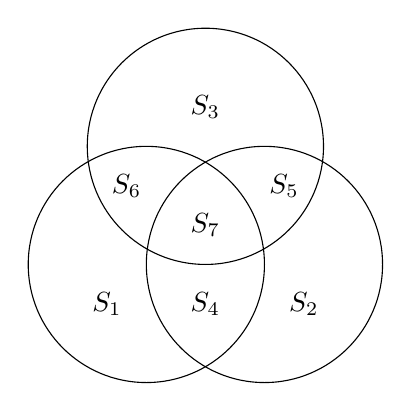
\begin{tikzpicture}
	\draw (0:-0.75cm) circle (1.5cm);
	\draw (90:1.5cm) circle (1.5cm);
	\draw (0:0.75cm) circle (1.5cm);
	\begin{scope}
    	\clip (0:-0.75cm) circle (1.5cm);
    	\clip (90:1.5cm) circle (1.5cm);
    	\clip (0:0.75cm) circle (1.5cm);
		\end{scope}
        \node at (-1.25,-0.5) {$S_1$};
        \node at (1.25,-0.5) {$S_2$};
        \node at (0,2) {$S_3$};
        \node at (0,-0.5) {$S_4$};
        \node at (1, 1.) {$S_5$};
        \node at (-1, 1.) {$S_6$};
        \node at (0,0.5){$S_7$};
    \end{tikzpicture}

    \hspace{1.3em}
    Let $A=\bigcup\set{S_1,S_4,S_6,S_7}, B=\bigcup\set{S_3,S_5,S_6,S_7}, C=\bigcup\set{S_2,S_4,S_5,S_7}$, 
    where $\forall i,j\in\set{1,2,...,7}, S_i\cap S_j=\varnothing$.

    \vspace{0.5em} \hspace{1.3em}
    First we prove \underline{the lemma} that for $A,B,C\subseteq X$, it holds that   

    \vspace{-1.5em}
    $$|A\cap C|\cdot |B\cup C| + |A\cup C| \cdot |B\cap C| \leq |C| \cdot(|A| + |B|) $$

    \vspace{-0.5em} \hspace{1.3em}
    The proof is as follows.

    \vspace{-3em}
    \begin{align*}
        &|A\cap C|\cdot |B\cup C| + |A\cup C| \cdot |B\cap C| \leq |C| \cdot(|A| + |B|) \\
        \Longleftrightarrow\ & \left(|S_6|+|S_7|\right)\cdot\left(|S_2|+|S_4|+|S_5|+|S_7|+|S_3|+|S_6|\right) +\\
        & \left(|S_4|+|S_7|\right)\cdot\left(|S_1|+|S_4|+|S_6|+|S_7|+|S_3|+|S_5|\right) \\
        & \le \left(|S_3|+|S_5|+|S_6|+|S_7|\right)\cdot\left(|S_1|+|S_4|+|S_6|+|S_7|+|S_2|+|S_4|+|S_5|+|S_7|\right) \\
        \Longleftrightarrow\ & \left(|S_6|+|S_7|\right)\cdot|S_3|+\left(|S_4|+|S_7|\right)\cdot\left(|S_5|+|S_6|\right) \\
        & \le \left(|S_3|+|S_5|\right)\left(|S_2|+|S_4|+|S_5|+|S_7|+|S_6|\right)+\left(|S_6|+|S_7|\right)\left(|S_1|+|S_4|+|S_7|\right) \\
        \Longleftrightarrow\ &0\le |S_3|\cdot|S_2|+|S_3|\cdot|S_4|+|S_3|\cdot|S_5|+|S_2|\cdot|S_5|+|S_5|^2+ \\
        &|S_5|\cdot|S_6|+|S_6|\cdot|S_1|+|S_7|\cdot|S_1|+|S_7|\cdot|S_4|+|S_7|^2 \text{ (Always Holds.)}
    \end{align*}

    \hspace{1.3em}
    Moreover, we have $|A\cup C|\cdot|B\cup C|\geq |A\cup B|\cdot|C|$. (The proof is as follows.)

    \vspace{-3em}
    \begin{align*}
        &|A\cup C|\cdot|B\cup C|\geq |A\cup B|\cdot|C|\\
        \Longleftrightarrow\ &\left(|S_1|+|S_4|+|S_6|+|S_7|+|S_3|+|S_5|\right)\cdot\left(|S_2|+|S_4|+|S_5|+|S_7|+|S_3|+|S_6|\right)\\
        & \geq \left(|S_1|+|S_4|+|S_6|+|S_7|+|S_2|+|S_5|\right)\cdot\left(|S_3|+|S_5|+|S_6|+|S_7|\right)\\
        \Longleftrightarrow\ & |S_3|\cdot\left(|S_2|+|S_4|+|S_5|+|S_7|+|S_3|+|S_6|\right) + \left(|S_1|+|S_4|+|S_6|+|S_7|+|S_5|\right)\cdot\left(|S_2|+|S_4|\right)\\
        &\geq |S_2|\cdot\left(|S_3|+|S_5|+|S_6|+|S_7|\right) \\
        \Longleftrightarrow\ & \left(|S_4|+|S_5|+|S_6|+|S_7|\right)\cdot\left(|S_3|+|S_4|\right) + |S_3|^2 + |S_2|\cdot\left(|S_1|+|S_4|\right) \geq 0
    \end{align*}

    \hspace{1.3em}
    Meanwhile, we have

    \vspace{-3em}
    \begin{align*}
        |A|+|B| &= |S_1|+|S_4|+|S_6|+|S_7|+|S_2|+|S_5| \\
        & = (|S_1|+|S_6|+|S_2|+|S_5|) + (|S_4|+|S_7|) = |A\cup B|+|A\cap B|
    \end{align*}

    \vspace{-0.75em} \hspace{1.3em}
    Then we know
    
    \vspace{-3em}
    \begin{align*}
        |A\cup B|\cdot\left(|A\cap C|\cdot|B\cup C|+|A\cup C|\cdot|B\cap C|\right) &\le |A\cup B|\cdot|C|\cdot\left(|A|+|B|\right) \\
        & = |A\cup B|\cdot|C|\cdot\left(|A\cap B|+|A\cup B|\right)  \\
        & \le |A\cup C|\cdot|B\cup C|\left(|A\cap B|+|A\cup B|\right) \\
        \text{i.e.}\qquad \dfrac{|A\cap C|}{|A\cup C|}+\dfrac{|B\cap C|}{|B\cup C|}\le \dfrac{|A\cap B|}{|A\cup B|}+1 \Longleftrightarrow & 1- \dfrac{|A\cap B|}{|A\cup B|} \le 1-\dfrac{|A\cap C|}{|A\cup C|}+1-\dfrac{|C\cap B|}{|C\cup B|} \\
        \Longleftrightarrow d(A,B)\le d(A,C)+d(C,B) \qquad \qquad\ 
   \end{align*}

   \vspace{-0.25em} \hspace{1.3em}
   Therefore, Jaccard distance is a metric.
\end{proof}

\vspace{1em}
\subsection{Cosine Distance is Not A Metric}
\vspace{1em}
\begin{disproof}
    Recall that cosine distance for $\bd{x},\bd{y}\in\mathbb{R}^d$ is

    \vspace{-0.75em}
    $$d(\bd{x},\bd{y}) = \frac{\sum_{i=1}^dx_iy_i}{\sqrt{\sum_{i=1}^dx_i^2}\sqrt{\sum_{i=1}^dy_i^2}}$$

    \hspace{2.6em}
    Obvious exists $\bd{x}=(1,1,1,1)$ and $\bd{y}=(-1,-1,-1,-1)$ s.t. $d(\bd{x},\bd{y})=-1<0$.

    \hspace{2.6em}
    Thus, cosine distance is not a metric.
\end{disproof}

\vspace{1em}
\subsection{Edit Distance is A Metric}
\vspace{1em}
\begin{proof}
    Recall that edit distance (Levenshtein Distance) for two strings $x$ and $y$ is

    \vspace{-1.5em}
    \begin{align*}
        \mathrm{lev}(x,y) = 
        \left\{
            \begin{array}{ll}
                |x|, & \text{if $|y|=0$} \\
                |y|, & \text{if $|x|=0$} \\
                \mathrm{lev}(x[1:], y[1:]), & \text{if $x[0]=y[0]$} \\
                1+\min\left\{
                        \mathrm{lev}(x[1:],y),
                        \mathrm{lev}(x,y[1:]),
                        \mathrm{lev}(x[1:],y[1:])
                \right\}
                &
                \text{otherwise}
            \end{array}
        \right.
    \end{align*}

    \hspace{1.3em}
    where $s[k:]$ means the string of all but the first $k$ characters of $s$.

    \vspace{1em} \hspace{1.3em}
    \textbf{Property 1.} By the definition of $\mathrm{lev}(\cdot)$, obvious for any string $x,y$, $\mathrm{lev}(x,y)\geq 0$.

    \hspace{1.3em}
    \textbf{Property 2.} For any string $x$, there is

    \vspace{-1em}
    $$\mathrm{lev}(x,x) = \mathrm{lev}(x[1:],x[1:]) = \mathrm{lev}(x[2:],x[2:]) = \dots = \mathrm{lev}(x\left[|x|:\right], x\left[|x|:\right]) = 0.$$

    \hspace{1.3em}
    \textbf{Property 3.} By the definition of edit distance, it is obvious that $\mathrm{lev}(x,y)={lev}(y,x)$.

    \hspace{1.3em}
    \textbf{Property 4.} For any string $x$, $y$ and $z$, $\mathrm{lev}(x,y)\le \mathrm{lev}(x,z)+\mathrm{lev}(z,y).$ The proof is as follows.

    \hspace{1.3em} We prove Property 4 by contradiction.

    \hspace{1.3em}
    Assume exist $x,y,z$ s.t. $\mathrm{lev}(x,y)>\mathrm{lev}(x,z)+\mathrm{lev}(z,y).$

    \hspace{1.3em}
    Consider the arguments of $\mathrm{lev}(\cdot)$ when recursively calculate $\mathrm{lev}(x,y), \mathrm{lev}(x,z), \mathrm{lev}(z,y)$. Then we get three sequences, $x \to a_1 \to a_2 \to \dots \to a_N \to y$, $x \to b_1 \to b_2 \to \to \dots b_M \to z$, $z \to c_1 \to c_2 \to \dots \to c_K \to y$, which in fact tell us how to change $x$ to $y$, $x$ to $z$, $z$ to $y$ respectively. 

    \hspace{1.3em}
    By the meaning of edit distance, we know $\mathrm{lev}(x,y), \mathrm{lev}(x,z), \mathrm{lev}(z,y)$ are costs when we change $x \to a_1 \to a_2 \to \dots \to a_N \to y$, $x \to b_1 \to b_2 \to \dots \to b_M \to z$, $z \to c_1 \to c_2 \to \dots \to c_K \to y$ respectively. Moreover, $x \to a_1 \to a_2 \to \dots a_N \to y$ is the way to change $x$ to $y$ with the minimal cost.

    \hspace{1.3em}
    Meanwhile, there exists a sequence $x\to b_1 \to b_2 \to \dots \to b_M \to z \to c_K \to \dots \to c_2 \to c_1 \to y$ with cost $\mathrm{lev}(x,z)+\mathrm{lev}(z,y)<\mathrm{lev}(x,y)$. \underline{\textbf{Contradiction!}}

    \vspace{1em} \hspace{1.3em}
    In conclusion, edit distance is a metric.
\end{proof}

\vspace{1em}
\subsection{Hamming Distance is A Metric}
\vspace{1em}
\begin{proof}
    Recall that Hamming distance for two strings $x$ and $y$ with the same length $L$ is

    \vspace{-0.75em}
    $$d(x,y) = \sum_{i=1}^L \mathbbm{1}[x_i\neq y_i]$$

    \hspace{1.3em}
    \textbf{Property 1.} Obvious for any string $x,y$, $d(x,y)\geq 0$.

    \hspace{1.3em}
    \textbf{Property 2.} For any string $x$, $d(x,x)=\sum_{i=1}^L 0 = 0.$

    \hspace{1.3em}
    \textbf{Property 3.} For any string $x$ and $y$, $d(x,y)=\sum_{i=1}^L \mathbbm{1}[x_i\neq y_i] = \sum_{i=1}^L \mathbbm{1}[y_i\neq x_i] = d(y,x)$.

    \hspace{1.3em}
    \textbf{Property 4.} For any string $x$, $y$ and $z$, $d(x,y)\le d(x,z)+d(z,y).$ The proof is as follows.

    \hspace{1.3em}
    First we prove that $\mathbbm{1}[a\neq b] \le \mathbbm{1}[a\neq c] + \mathbbm{1}[c\neq b]$ for any char $a,b,c$ by contradiction.

    \hspace{1.3em}
    Assume exists $a,b,c$ s.t. $\mathbbm{1}[a\neq b] \le \mathbbm{1}[a\neq c] + \mathbbm{1}[c\neq b]$. 
    
    \hspace{1.3em}
    The only possible case is that $\mathbb{1}[a\neq b]=1$ and $\mathbbm{1}[a\neq c] = \mathbbm{1}[c\neq b] = 0.$

    \hspace{1.3em}
    Then we get $a\neq b$ and $a=c=b$. \underline{\textbf{Contradiction!}}

    \vspace{1em} \hspace{1.3em}
    Further, we have 

    \vspace{-2em}
    \begin{align*}
        d(x,y) &= \sum_{i=1}^L \mathbbm{1}[x_i\neq y_i] \le \sum_{i=1}^L \mathbbm{1}[x_i\neq z_i] + \mathbbm{1}[z_i\neq y_i] \\
        &= \sum_{i=1}^L \mathbbm{1}[x_i\neq z_i] + \sum_{i=1}^L \mathbbm{1}[z_i\neq y_i] =  d(x,z) + d(z,y)
    \end{align*}

    \hspace{1.3em}
    Therefore, Hamming Distance is a metric.
\end{proof}

\vspace{3em}
\section{Average Distance Between A Pair Of Points}
\vspace{1em}
\begin{proof}
    Let the line of length $L$ be $AB$. Let the pair of points be $M$ and $N$. Let $x\triangleq|AM|, y\triangleq|AN|$.

    \hspace{1.3em}
    Obvious $x,y\sim \mathcal{U}(0,L)$.

    \vspace{-2em} \hspace{1.3em}
    \begin{align*}
        \staExp{}{|x-y|} &= \int_0^L \frac{1}{L^2}\cdot x\cdot\sqrt{2}(L-x)\cdot\frac{\sqrt{2}}{2}\mathrm{d}x + \int_0^L \frac{1}{L^2}\cdot y\cdot\sqrt{2}(L-y)\cdot\frac{\sqrt{2}}{2}\mathrm{d}y \\
        &= \frac{2}{L^2} \int_0^L x(L-x) \mathrm{d}x = \frac{2}{L^2} \left(\frac{1}{2}L^3-\frac{1}{3}L^3\right) \\
        &= \frac{1}{3}L
    \end{align*}

    \vspace{-0.5em} \hspace{1.3em}
    Thus, the average distance between a pair of points is $\dfrac{1}{3}L$.
\end{proof}

\vspace{1em}
\section{Eckart-Young-Mirsky Theorem}

Let $\bd{A} = \bd{U}\bd{\Sigma}\bd{V}^\top$ and $\bd{B} = \bd{U} \bd{S} \bd{V}^\top$ where $\bd{S} = $ diagonal $r \times r$ matrix with $s_i=\left\{
    \begin{array}{ll}
        \sigma_i & \text{if } i=1,2,...,k\\
        0 & \text{otherwise}
    \end{array}
    \right.$

\vspace{0.5em} \hspace{-1.8em}
Prove that $\bd{B}$ is one of the best $k$-rank approximations to $\bd{A}$ in terms of Frobenius norm error.


\vspace{2em}

\begin{proof}
    Let $\bd{A}\in\mathbb{R}^{m\times n}$. To prove the proposition, we just need to prove that

    \vspace{-1em}
    $$\text{for any }\bd{C}\in\set{\bd{X}\in\mathbb{R}^{m\times n}\mid\mathtt{rank}(\bd{X})=k},\ \underset{\bd{C}}{\min}\|\bd{A}-\bd{C}\|_F=\|\bd{A}-\bd{B}\|_F.$$

    \vspace{1em} \hspace{1.3em}
    First we prove the following lemma.

    \hspace{1.3em}
    \underline{Lemma.} For any matrix $\bd{A}\in\mathbb{R}^{m'\times n'}$ and $\bd{W}\in\mathbb{R}^{p'\times n'}$ s.t. $\bd{W}^\top\bd{W}=\bd{I}$, $\|\bd{A}\bd{W}^\top\|_F=\|\bd{A}\|_F.$

    \hspace{5.1em} For any matrix $\bd{A}\in\mathbb{R}^{m'\times n'}$ and $\bd{V}\in\mathbb{R}^{m'\times p'}$ s.t. $\bd{V}^\top\bd{V}=\bd{I}$, $\|\bd{V}\bd{A}\|_F=\|\bd{A}\|_F.$

    \hspace{1.3em}
    The proof for the lemma is as follows.

    \vspace{-2.5em}
    \begin{align*}
        \|\bd{A}\bd{W}^\top\|_F &= \sqrt{\mathtt{tr}\left(\left(\bd{A}\bd{W}^\top\right)^\top\bd{A}\bd{W}^\top\right)} = \sqrt{\mathtt{tr}\left(\bd{W}\bd{A}^\top\bd{A}\bd{W}^\top\right)} = \sqrt{\mathtt{tr}\left(\bd{A}^\top\bd{A}\bd{W}^\top\bd{W}\right)} \\
        &= \sqrt{\mathtt{tr}\left(\bd{A}^\top\bd{A}\bd{I}\right)} = \sqrt{\mathtt{tr}\left(\bd{A}^\top\bd{A}\right)} = \|\bd{A}\|_F \quad\text{ where $\bd{I}$ is identity matrix.}\\
        \|\bd{V}\bd{A}\|_F^2 &= \sqrt{\mathtt{tr}\left(\left(\bd{VA}\right)^\top\bd{VA}\right)} = \sqrt{\mathtt{tr}\left(\bd{A}^\top\bd{V}^\top\bd{V}\bd{A}\right)} = \sqrt{\mathtt{tr}\left(\bd{A}^\top\bd{I}\bd{A}\right)} \\
        &= \sqrt{\mathtt{tr}\left(\bd{A}^\top\bd{A}\right)} = \|\bd{A}\|_F
    \end{align*}

    \vspace{-3.3em} \hspace{26em}
    where $\bd{I}$ is identity matrix. \whiteqed

    \vspace{3em} \hspace{1.3em}
    By the lemma, we know 
    
    \vspace{-2.5em}
    \begin{align*}
        \|\bd{A}-\bd{B}\|_F^2 & = \|\bd{U}\left(\bd{\Sigma}-\bd{S}\right)\bd{V}^\top\|_F^2 = \|\bd{\Sigma}-\bd{S}\|_F^2 = \sum_{i=1}^r (\sigma_i-s_i)^2 = \sum_{i=k+1}^r \sigma_i^2.
    \end{align*}

    \hspace{1.3em}
    Now we just need to prove that

    \vspace{-1em}
    $$\text{for any }\bd{C}\in\set{\bd{X}\in\mathbb{R}^{m\times n}\mid\mathtt{rank}(\bd{X})=k},\ \underset{\bd{C}}{\min}\|\bd{A}-\bd{C}\|_F^2=\sum_{i=k+1}^r \sigma_i^2.$$
    
    \vspace{-0.5em} \hspace{1.3em}
    By SVD Theorem, we know there exist matrices $\widetilde{\bd{U}}, \widetilde{\bd{V}}$ and an $r\times r$ diagonal matrix $\bd{\Gamma}=\mathtt{diag}\left(\gamma_1,\gamma_2,...\gamma_k,0,...,0\right)$ s.t. $\bd{C}=\widetilde{\bd{U}}\bd{\Gamma}\widetilde{\bd{V}}^\top$. By the lemma, we know $\|\bd{C}\|_F = \sum_{i=1}^r \gamma_i^2$.
    
    \hspace{1.3em}
    Let $\hat{\bd{U}}=\bd{U}^\top\widetilde{\bd{U}} = \left(\hat{\bd{u}}_1,\hat{\bd{u}}_2,...,\hat{\bd{u}}_r\right)^\top, \hat{\bd{V}}^\top = \bd{V}^\top \widetilde{\bd{V}} = \left(\hat{\bd{v}}_1,\hat{\bd{v}}_2,...,\hat{\bd{v}}_r\right)$.

    \hspace{1.3em}
    Obvious $\hat{\bd{U}}$ is orthogonal since $\hat{\bd{U}}^\top\hat{\bd{U}}=\widetilde{\bd{U}}^\top\bd{U}\bd{U}^\top\widetilde{\bd{U}} = \widetilde{\bd{U}}^\top\widetilde{\bd{U}} = \bd{I}$. Similarly, $\hat{\bd{V}}$ is orthogonal.

    \hspace{1.3em}
    Then we have

    \vspace{-2em}
    \begin{align*}
        \langle \bd{A}, \bd{C} \rangle & = \mathtt{tr}\left(\bd{V}\bd{\Sigma}^\top\bd{U}^\top\widetilde{\bd{U}}\bd{\Gamma}\widetilde{\bd{V}}^\top\right) = \mathtt{tr}\left(\bd{\Sigma}^\top\bd{U}^\top\widetilde{\bd{U}}\bd{\Gamma}\widetilde{\bd{V}}^\top\bd{V}\right) = \mathtt{tr}\left(\bd{\Sigma}^\top\hat{\bd{U}}\bd{\Gamma}\hat{\bd{V}}^\top\right) \\
        & = \sum_{i=1}^k \sigma_i\gamma_i\hat{\bd{u}}_i^\top \hat{\bd{v}}_i 
        \le \sum_{i=1}^k \sigma_i\gamma_i\|\hat{\bd{u}}_i\|\|\hat{\bd{v}}_i\| = \sum_{i=1}^k \sigma_i\gamma_i.
    \end{align*}

    \hspace{1.3em}
    Thus, we have 

    \vspace{-2em}
    \begin{align*}
        \|\bd{A}-\bd{C}\|_F^2 & = \mathtt{tr}\left(\left(\bd{A}-\bd{C}\right)^\top\left(\bd{A}-\bd{C}\right)\right) = \mathtt{tr}\left(\bd{A}^\top\bd{A}-\bd{A}^\top\bd{C}-\bd{C}^\top\bd{A}+\bd{C}^\top\bd{C}\right) \\
        & = \mathtt{tr}\left(\bd{A}^\top\bd{A}\right) - 2\langle \bd{A}, \bd{C} \rangle + \mathtt{tr}\left(\bd{C}^\top\bd{C}\right) = \|\bd{A}\|_F - 2\langle\bd{A},\bd{C}\rangle + \|\bd{C}\|_F \\
        &\geq \sum_{i=1}^r \sigma_i^2 - 2\sum_{i=1}^k \sigma_i\gamma_i + \sum_{i=1}^k \gamma_i^2 = \sum_{i=k+1}^r \sigma_i^2 + \sum_{i=1}^k \left(\sigma_i-\gamma_i\right)^2 \\
        & \geq \sum_{i=k+1}^r \sigma_i^2.
    \end{align*}

    \hspace{1.3em}
    Therefore, $\bd{B} = \bd{U} \bd{S} \bd{V}^\top$ is one of the best $k$-rank approximations to $\bd{A}$ in terms of Frobenius norm error.
\end{proof}


\vspace{1em}
\section{Average Jaccard Similarity of Two Randomly-Sampled Sets}
\vspace{1em}

\begin{solution}
    Let $J(A,B)$ be the Jaccard similarity of set $A$ and $B$.

    \vspace{0.5em} \hspace{2.5em}
    Totally, there are $\dbinom{n}{m}\cdot\dbinom{n}{m}$ possible pairs of $(S,T)$.

    \vspace{0.5em} \hspace{2.5em}
    It is obvious that $\max\left\{0,2m-n\right\}\le |S\cap T| \le m.$
    
    \vspace{0.5em} \hspace{2.5em}
    When $|S\cap T|=k$, there are $\dbinom{n}{k}\cdot\dbinom{n-k}{m-k}\cdot\dbinom{n-m}{m-k}$ possible pairs of $(S,T)$. 
    
    \vspace{0.5em} \hspace{2.5em}
    In this case, the Jaccard similarity of $S$ and $T$ is $\dfrac{k}{2m-k}.$


    \hspace{2.5em}
    Thus,
    
    \vspace{-1em}
    \begin{align*}
        \staExp{}{J(S,T)} = \sum_{k=\max\left\{0,2m-n\right\}}^{m}\frac{\dbinom{n}{k}\cdot\dbinom{n-k}{m-k}\cdot\dbinom{n-m}{m-k}}{\dbinom{n}{m}^2}\cdot\frac{k}{2m-k}.
    \end{align*}

    




\end{solution}

% Suppose we have a universal set U of n elements, and we choose two subsets S and T at random, each with m of the n elements. What is the expected value of the Jaccard similarity of S and T ?  A sum expression of the expectation is acceptable if you can't simplify it.

\end{document}
